\pagebreak
\section{Introduction}
In this project you will simulate supersonic flow through a two-dimensional scramjet engine, using a first-order, adaptive, finite-volume method. Combustion will not be included, and your investigation will focus on measuring the total pressure recovery of the engine. The shock structure inside the engine is complex, and accurate simulations will require adapted meshes to resolve the shocks and expansions.

\paragraph{Geometry:} Figure \ref{fig:engine_geometry} shows the geometry of the engine, which consists of two sections: lower and upper. The reference length is the height of the engine channel at the exit, which is d = 1. Note that the units of the measurements are not relevant, as you will be reporting non-dimensional quantities.

\begin{figure}[h]
    \centering
    \includegraphics[width = 0.75\linewidth]{admin/engine_geometry.png}
    \caption[Engine Geometry and Boundary Conditions]{Engine geometry and boundary conditions.}
    \label{fig:engine_geometry}
\end{figure}

\paragraph{Governing Equations:} Use the two-dimensional Euler equations, with a ratio of specific heats of $\gamma = 1.4$.

\paragraph{Units:} To avoid ill-conditioning, use ``convenient'' $\mathcal{O}(1)$ units for this problem, in which the freestream state is

\begin{equation}\label{eqn:flow}
    \bf{u}_{\infty} = \begin{bmatrix} \rho, & \rho u, & \rho v, & \rho E \end{bmatrix}^{T} = \begin{bmatrix}
        1, & M_\infty\cos{(\alpha)}, & M_\infty\sin{(\alpha)}, & \frac{1}{\gamma(\gamma-1)} + \frac{M_\infty^2}{2}
    \end{bmatrix}^T
\end{equation}\myequations{Freestream State}

where $M_\infty$ is the free-stream Mach number, and $\alpha$ is the angle of attack.

\paragraph{Initial and Boundary Conditions:} The computational domain consists of the region around the engine. The inflow portion of the far-field rectangle consists of the left and bottom boundaries. On these boundaries apply free-stream ``full-state'' conditions, with a free-stream Mach number of $M_\infty = 2.2$. You will investigate angles of attack in the range $\alpha \in [0, 3\degree]$, with a baseline value of $\alpha = 1\degree$. On the outflow and engine exit boundaries, assume that the flow is supersonic, which means that no boundary state is needed -- the flux is computed from the interior state. On the engine surface, apply the inviscid wall boundary condition.

When initializing the state in a new run, i.e. not when restarting from an existing state, you can set all cells to the same state, based on the free-stream Mach number, $M_\infty$.


\paragraph{Output:} Shocks inside the engine are necessary to slow the flow down and compress it for combustion, but they also lead to a loss in total pressure (lost work). A figure of merit is then the
\textit{average total pressure recovery} (ATPR), defined by an integral of the engine exit of the ratio of the
total pressure to the freestream total pressure,

\begin{equation}\label{eqn:ATPR}
    \text{ATPR} = \frac{1}{d}\int_0^d\frac{p_t}{p_{t,\infty}}\ dy,\quad p_t = p\left(1 + \frac{\gamma - 1}{2}M^2\right)^{\gamma/(\gamma-1)},
\end{equation}\myequations{Average Total Pressure Recovery}

where $p$ is the pressure, $p_t$ is the total pressure, and $y$ measures the vertical distance along the engine exit.


\pagebreak
\section{Numerical Method}
Use the first-order finite volume methods to solve for the flow through the engine. March the solution to steady state using local time stepping, starting from either an initial uniform flow, or from an existing converged or partially-converged state.

\paragraph{Discretization:} From the notes, cell $i$'s average, $(\bf{u}_i)$, evolves in time according to

\begin{equation}\label{eqn:cell_avg}
    A_i\frac{d\bf{u}_i}{dt} + {\bf{R}_i = 0} \rightarrow \frac{d{\bf{u}_i}}{dt} = -\frac{1}{A_i}\bf{R}_i.
\end{equation}\myequations{Cell Average}

where the flux residual $\bf{R}_i$ for a triangular cell is

\begin{equation}\label{eqn:flux_residual}
    {\bf{R}_i} = \sum_{e=1}^{3} {\bf{\hat{F}(u_i,u_{N({i,e})}}},\vec{n}_{i,e})\Delta l_{i,e}
\end{equation}\myequations{Flux Residual}

Recall that $N(i,e)$ is the cell adjacent to cell $i$ across edge $e$, and $\vec{n}_{i,e} , \Delta l_{i,e}$ are the outward normal and length on edge $e$ of cell $i$. Discretize Equation \ref{eqn:cell_avg} with forward Euler time integration and use local time stepping to drive the solution to steady state.

\paragraph{Local Time Stepping:} To implement local time stepping, a vector of time steps is calculated,
one time step for each cell: $\Delta t_i$. Defining the CFL number for cell $i$ as,

\begin{equation}\label{eqn:CFL}
    \text{CFL}_i = \frac{\Delta t_i}{2A_i}\sum_{e=1}^{3}|s|_{i,e}\Delta l_{i,e},
\end{equation}\myequations{CFL Definition}

where $A_i$ is the area of the cell, the summation is over the three edges of a cell, and $|s|_{i,e}$ is the
maximum propagation speed for edge $e$.

Time stepping requires the value of $\Delta t_i/A_i$ for each cell, and this can be calculated by re-arranging
Equation \ref{eqn:CFL},

\begin{equation}\label{eqn:time_stepping}
    \frac{\Delta t_i}{A_i} = \frac{2\text{CFL}_i}{\sum_{e=1}^{3}|s|_{i,e}\Delta l_{i.e}}.
\end{equation}\myequations{Time Stepping}

\pagebreak
The easiest method to calculate the right-hand-side is to calculate the summation of $|s|_e \Delta l_{i,e}$ during the flux evaluations. Note that the propagation speed $|s|_{i,e}$ should be calculated by the flux function. In local time stepping, the CFL number for each cell is the same: $\text{CFL}_i = \text{CFL} = 1.0$ is a good choice for this project.

\paragraph{Residuals and Convergences:} Assess convergence by monitoring the undivided $L_1$ norm of the residual vector, defined as

\begin{equation}\label{eqn:residual_vector}
    |{\bf R}|_{L_1} = \sum_{\text{cells}\ i} \sum_{\text{states}\ k}|R_{i,k}|
\end{equation}\myequations{Residual Vector}

That is, take the sum of the absolute values of all of the entries in your residual vector (you will be summing the 4 conservation equation residuals in each cell). You should not divide by the number of entries/cells, as the residuals already represent integrated quantities over the cells, so the sum will behave properly with mesh refinement. Deem a solution converged when $|{\bf R}|_{L_1} < 10^{-5}$.

\paragraph{Numerical Flux:} Use the Roe flux for the interface flux and to impose the full-state far-field boundary condition. This flux is described in the course notes. You will need to verify your flux once implemented, using the following tests:

\begin{itemize}
    \item Consistency check: ${\bf F(u_L, u_L}, \vec{n})$ should be the same as $ {\bf \vec{F}(U_L)}\cdot \vec{n}$ (the analytical flux dotted with the normal).
    \item Flipping the direction: check that $ {\bf F(u_L, u_R} , \vec{n} ) =  {\bf-F(u_R , u_L }, -\vec{n} )$.
    \item States with supersonic normal velocity: the flux function should return the analytical flux from the upwind state. The downwind state should not have any effect on flux.
\end{itemize}


\paragraph{Time Stepping:} Use the forward-Euler method to drive the solution to steady state. With local
time-stepping, the update on cell $i$ at iteration $n$ can be written as

\begin{equation}\label{eqn:forward_euler}
    {\bf u}_i^{n+1} = {\bf u}_i^n - \frac{\Delta t_i^n}{A_i}{\bf R_i(U^n)},
\end{equation}\myequations{Forward-Euler Time Stepping Scheme}

where $\Delta t^n_i$ is the local time step computed from the state at time step $n$.

\pagebreak
\paragraph{Mesh:} You are provided with a baseline mesh of 1670 cells, shown in Figure \ref{fig:baseline_mesh}. This mesh will not provide very accurate flow solutions, but it will serve as the starting point for adaptation. The included {\texttt{readme.txt}} file describes the structure of the text-based {\texttt{.gri}} mesh file. You are also given python and Matlab codes for reading the {\texttt{.gri}} mesh file and for plotting/processing the mesh.

\begin{figure}[h]
    \centering
    \includegraphics[width = 0.75\linewidth]{admin/baseline_mesh.pdf}
    \caption[Scramjet Baseline Mesh]{Scramjet baseline mesh.}
    \label{fig:baseline_mesh}
\end{figure}

\paragraph{Output Calculation:} The average total pressure recovery output in Equation \ref{eqn:ATPR} requires an integral over the engine exit. Approximate this integral by summing over the edges on the exit boundary. For each edge, use the state from the adjacent cell to calculate the total pressure.


\pagebreak
\section{Adaptation}
You will use mesh adaptation to improve solution quality. Adapting a mesh means locally increasing the mesh resolution in regions where errors are likely to be large. This requires a measurement of error and a method for adapting the mesh. A reasonable way to measure error is to look at jumps in the solution between cells. For example, looking at jumps in the Mach number, we can define an error indicator for each interior edge $e$ according to

\begin{equation*}
    \text{interior:}\ \epsilon_e = |M_{k^+} - M_{k^-}|h_e.
\end{equation*}

In this formula, $M_{k^+}$ and $M_{k^-}$ are the Mach numbers on the two cells adjacent to edge $e$, and $h_e$ is the length of edge $e$.

You can assume that the error indicator on the farfield boundary edges is zero. On the engine boundary (solid wall), define the error indicator by

\begin{equation*}
    \text{wall:}\ \epsilon_e = |M_k^\perp|h_e,
\end{equation*}

where $M_k^\perp$ is the Mach number of the cell’s velocity component in the edge normal direction.

After calculating the error indicators $\epsilon_e$ over all edges (interior and boundary), sort the indicators in decreasing order and flag a small fraction $f = .03$ of edges with the highest error for refinement. Next, to smooth out the refinement pattern, loop over all cells: if a cell has \textit{any} of its edges flagged for refinement, then flag \textit{all} of its edges for refinement. This will increase the total number of edges for refinement.


Once edges are flagged as described, refine all cells adjacent to flagged edges. These cells will fall
into one of three categories, shown in Figure \ref{fig:triangle_refinement}, and they should be refined as indicated. At each adaptive iteration, transfer the solution to the new mesh to provide a good initial guess for the next solve.

\begin{figure}[h]
    \centering
    

\tikzset{every picture/.style={line width=0.75pt}} %set default line width to 0.75pt        

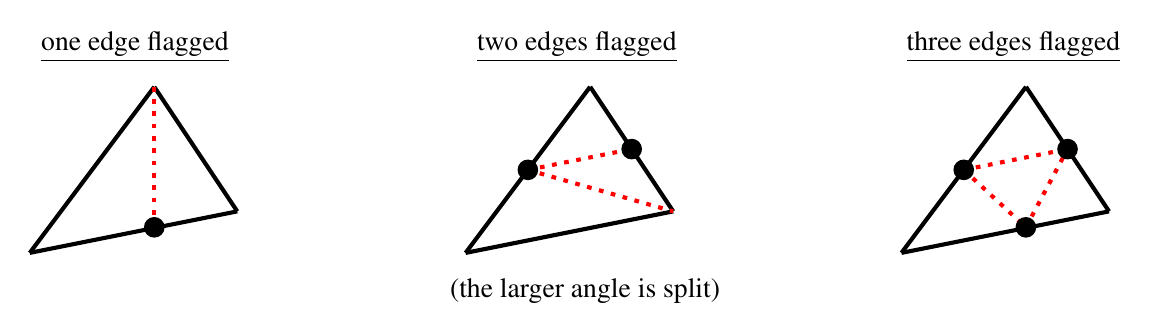
\begin{tikzpicture}[x=0.75pt,y=0.75pt,yscale=-1,xscale=1]
%uncomment if require: \path (0,300); %set diagram left start at 0, and has height of 300

%Straight Lines [id:da36192842191098795] 
\draw [line width=1.5]    (60,160) -- (120,80) ;
%Straight Lines [id:da5425661526994696] 
\draw [line width=1.5]    (120,80) -- (160,140) ;
%Straight Lines [id:da44878431831371346] 
\draw [line width=1.5]    (160,140) -- (60,160) ;
%Straight Lines [id:da0011262443709205705] 
\draw [line width=1.5]    (270,160) -- (330,80) ;
%Straight Lines [id:da21951601188615122] 
\draw [line width=1.5]    (330,80) -- (370,140) ;
%Straight Lines [id:da9300714537435593] 
\draw [line width=1.5]    (370,140) -- (270,160) ;
%Straight Lines [id:da3376367418061297] 
\draw [line width=1.5]    (480,160) -- (540,80) ;
%Straight Lines [id:da2556881107384765] 
\draw [line width=1.5]    (540,80) -- (580,140) ;
%Straight Lines [id:da7616804642146637] 
\draw [line width=1.5]    (580,140) -- (480,160) ;
%Straight Lines [id:da4163633440661523] 
\draw [color={rgb, 255:red, 255; green, 0; blue, 0 }  ,draw opacity=1 ][line width=1.5]  [dash pattern={on 1.69pt off 2.76pt}]  (120,80) -- (120,147.69) ;
%Straight Lines [id:da007547566900241609] 
\draw [color={rgb, 255:red, 255; green, 0; blue, 0 }  ,draw opacity=1 ][line width=1.5]  [dash pattern={on 1.69pt off 2.76pt}]  (300,120) -- (350,110) ;
%Straight Lines [id:da21236386256097184] 
\draw [color={rgb, 255:red, 255; green, 0; blue, 0 }  ,draw opacity=1 ][line width=1.5]  [dash pattern={on 1.69pt off 2.76pt}]  (300,120) -- (370,140) ;
%Straight Lines [id:da04751621039067011] 
\draw [color={rgb, 255:red, 255; green, 0; blue, 0 }  ,draw opacity=1 ][line width=1.5]  [dash pattern={on 1.69pt off 2.76pt}]  (510,120) -- (539.93,147.69) ;
%Straight Lines [id:da0959709459132021] 
\draw [color={rgb, 255:red, 255; green, 0; blue, 0 }  ,draw opacity=1 ][line width=1.5]  [dash pattern={on 1.69pt off 2.76pt}]  (539.93,147.69) -- (560,110) ;
%Straight Lines [id:da17305312497337466] 
\draw [color={rgb, 255:red, 255; green, 0; blue, 0 }  ,draw opacity=1 ][line width=1.5]  [dash pattern={on 1.69pt off 2.76pt}]  (510,120) -- (560,110) ;
%Shape: Circle [id:dp6356305041815642] 
\draw  [fill={rgb, 255:red, 0; green, 0; blue, 0 }  ,fill opacity=1 ] (115.54,147.69) .. controls (115.54,145.22) and (117.53,143.22) .. (120,143.22) .. controls (122.47,143.22) and (124.46,145.22) .. (124.46,147.69) .. controls (124.46,150.15) and (122.47,152.15) .. (120,152.15) .. controls (117.53,152.15) and (115.54,150.15) .. (115.54,147.69) -- cycle ;
%Shape: Circle [id:dp6939765362470538] 
\draw  [fill={rgb, 255:red, 0; green, 0; blue, 0 }  ,fill opacity=1 ] (295.54,120) .. controls (295.54,117.53) and (297.53,115.54) .. (300,115.54) .. controls (302.47,115.54) and (304.46,117.53) .. (304.46,120) .. controls (304.46,122.47) and (302.47,124.46) .. (300,124.46) .. controls (297.53,124.46) and (295.54,122.47) .. (295.54,120) -- cycle ;
%Shape: Circle [id:dp9518974624791348] 
\draw  [fill={rgb, 255:red, 0; green, 0; blue, 0 }  ,fill opacity=1 ] (345.54,110) .. controls (345.54,107.53) and (347.53,105.54) .. (350,105.54) .. controls (352.47,105.54) and (354.46,107.53) .. (354.46,110) .. controls (354.46,112.47) and (352.47,114.46) .. (350,114.46) .. controls (347.53,114.46) and (345.54,112.47) .. (345.54,110) -- cycle ;
%Shape: Circle [id:dp5417462498770167] 
\draw  [fill={rgb, 255:red, 0; green, 0; blue, 0 }  ,fill opacity=1 ] (505.54,120) .. controls (505.54,117.53) and (507.53,115.54) .. (510,115.54) .. controls (512.47,115.54) and (514.46,117.53) .. (514.46,120) .. controls (514.46,122.47) and (512.47,124.46) .. (510,124.46) .. controls (507.53,124.46) and (505.54,122.47) .. (505.54,120) -- cycle ;
%Shape: Circle [id:dp27821656516619253] 
\draw  [fill={rgb, 255:red, 0; green, 0; blue, 0 }  ,fill opacity=1 ] (555.54,110) .. controls (555.54,107.53) and (557.53,105.54) .. (560,105.54) .. controls (562.47,105.54) and (564.46,107.53) .. (564.46,110) .. controls (564.46,112.47) and (562.47,114.46) .. (560,114.46) .. controls (557.53,114.46) and (555.54,112.47) .. (555.54,110) -- cycle ;
%Shape: Circle [id:dp49666970713488623] 
\draw  [fill={rgb, 255:red, 0; green, 0; blue, 0 }  ,fill opacity=1 ] (535.46,147.69) .. controls (535.46,145.22) and (537.46,143.22) .. (539.93,143.22) .. controls (542.39,143.22) and (544.39,145.22) .. (544.39,147.69) .. controls (544.39,150.15) and (542.39,152.15) .. (539.93,152.15) .. controls (537.46,152.15) and (535.46,150.15) .. (535.46,147.69) -- cycle ;

% Text Node
\draw (64,52) node [anchor=north west][inner sep=0.75pt]   [align=left] {\underline{{\fontfamily{ptm}\selectfont one edge flagged}}};
% Text Node
\draw (274,52) node [anchor=north west][inner sep=0.75pt]   [align=left] {\underline{{\fontfamily{ptm}\selectfont two edges flagged}}};
% Text Node
\draw (481,52) node [anchor=north west][inner sep=0.75pt]   [align=left] {\underline{{\fontfamily{ptm}\selectfont three edges flagged}}};
% Text Node
\draw (261,171) node [anchor=north west][inner sep=0.75pt]   [align=left] {{\fontfamily{ptm}\selectfont (the larger angle is split)}};


\end{tikzpicture}

    \caption[Refinement of Triangles Given Edge Splittings]{Refinement of triangles given edge splittings.}
    \label{fig:triangle_refinement}
\end{figure}